\documentclass{article}

\usepackage{fancyhdr}
\usepackage{extramarks}
\usepackage{amsmath}
\usepackage{amsthm}
\usepackage{amsfonts}
\usepackage{tikz}
\usepackage[plain]{algorithm}
\usepackage{algpseudocode}
\usepackage{graphicx}
\usetikzlibrary{automata,positioning}

%
% Basic Document Settings
%

\topmargin=-0.45in
\evensidemargin=0in
\oddsidemargin=0in
\textwidth=6.5in
\textheight=9.0in
\headsep=0.25in

\linespread{1.1}

\pagestyle{fancy}
\lhead{\hmwkAuthorName}
\chead{\hmwkClass\ (\hmwkClassInstructor\ \hmwkClassTime): \hmwkTitle}
\rhead{\firstxmark}
\lfoot{\lastxmark}
\cfoot{\thepage}

\renewcommand\headrulewidth{0.4pt}
\renewcommand\footrulewidth{0.4pt}

\setlength\parindent{0pt}

%
% Create Problem Sections
%

\newcommand{\enterProblemHeader}[1]{
    \nobreak\extramarks{}{Problem \arabic{#1} continued on next page\ldots}\nobreak{}
    \nobreak\extramarks{Problem \arabic{#1} (continued)}{Problem \arabic{#1} continued on next page\ldots}\nobreak{}
}

\newcommand{\exitProblemHeader}[1]{
    \nobreak\extramarks{Problem \arabic{#1} (continued)}{Problem \arabic{#1} continued on next page\ldots}\nobreak{}
    \stepcounter{#1}
    \nobreak\extramarks{Problem \arabic{#1}}{}\nobreak{}
}

\setcounter{secnumdepth}{0}
\newcounter{partCounter}
\newcounter{homeworkProblemCounter}
\setcounter{homeworkProblemCounter}{1}
\nobreak\extramarks{Problem \arabic{homeworkProblemCounter}}{}\nobreak{}

%
% Homework Problem Environment
%
% This environment takes an optional argument. When given, it will adjust the
% problem counter. This is useful for when the problems given for your
% assignment aren't sequential. See the last 3 problems of this template for an
% example.
%
\newenvironment{homeworkProblem}[1][-1]{
    \ifnum#1>0
        \setcounter{homeworkProblemCounter}{#1}
    \fi
    \section{Problem \arabic{homeworkProblemCounter}}
    \setcounter{partCounter}{1}
    \enterProblemHeader{homeworkProblemCounter}
}{
    \exitProblemHeader{homeworkProblemCounter}
}

%
% Homework Details
%   - Title
%   - Due date
%   - Class
%   - Section/Time
%   - Instructor
%   - Author
%

\newcommand{\hmwkTitle}{Homework\ \#1}
\newcommand{\hmwkDueDate}{September 13, 2019}
\newcommand{\hmwkClass}{CMSE 820}
\newcommand{\hmwkClassTime}{}
\newcommand{\hmwkClassInstructor}{Professor Yuying Xie}
\newcommand{\hmwkAuthorName}{\textbf{Boyao Zhu}}

%
% Title Page
%

\title{
    \vspace{2in}
    \textmd{\textbf{\hmwkClass:\ \hmwkTitle}}\\
    \normalsize\vspace{0.1in}\small{Due\ on\ \hmwkDueDate\ at 11:59pm}\\
    \vspace{0.1in}\large{\textit{\hmwkClassInstructor\ \hmwkClassTime}}
    \vspace{3in}
}

\author{\hmwkAuthorName}
\date{}

\renewcommand{\part}[1]{\textbf{\large Part \Alph{partCounter}}\stepcounter{partCounter}\\}

%
% Various Helper Commands
%

% Useful for algorithms
\newcommand{\alg}[1]{\textsc{\bfseries \footnotesize #1}}

% For derivatives
\newcommand{\deriv}[1]{\frac{\mathrm{d}}{\mathrm{d}x} (#1)}

% For partial derivatives
\newcommand{\pderiv}[2]{\frac{\partial}{\partial #1} (#2)}

% Integral dx
\newcommand{\dx}{\mathrm{d}x}

% Alias for the Solution section header
\newcommand{\solution}{\textbf{\large Solution}}

% Probability commands: Expectation, Variance, Covariance, Bias
\newcommand{\E}{\mathrm{E}}
\newcommand{\Var}{\mathrm{Var}}
\newcommand{\Cov}{\mathrm{Cov}}
\newcommand{\Bias}{\mathrm{Bias}}

\begin{document}

\maketitle

\pagebreak

\begin{homeworkProblem}
    Assume \(Y=X^T\beta+\epsilon\), where \( X \in \mathbb{R}^P \) is not random and  \( \epsilon \sim N(0,1)\).   Given i.i.d. data \{(\(x_1,y_1\)),...(\(x_n,y_n\))\}, we would like to estimate \(\beta\in\mathbb{R}^P\) through maximum likelihood framework.  Write down the joint log likelihood and compare it with least square method.
\\

    \textbf{Solution}

    Let us assume that the disturbances \(\epsilon_t\), which are the elements of the vector \(\epsilon=[\epsilon_1,\epsilon_2,...,\epsilon_t]'\), are distributed independently and identically according a normal distribution
   
    \[
    N(\epsilon_t,0,\sigma^2) = \frac{1}{\sqrt{2\pi\sigma^2}}\exp\Big\{\frac{-1}{2\sigma^2}(y_t-x_t^T\beta)^2\Big\}
    \]
    Then, if the vectors \(x_t\) are taken as data, the observations \(y_t\); \(t=1,...,T\) have density functions \(N(y_t;x_t^T\beta,\sigma^2)\) which are of the same form as those of the disturbances, and the likelihood function of \(\beta\) and \(\sigma^2\), based on the sample, is
    
    \[
    L=\prod_{T=1}^T N(y_t;x_t^T\beta,\sigma^2)=(2\pi\sigma^2)^{-T/2}\exp\Big\{ \frac{-1}{2\sigma^2}(y-X^T\beta)^T(y-X^T\beta)  \Big\}
    \]
    
    The logarithm of this function
    \[
    L^*(\beta,\sigma)=-\frac{T}{2}\ln(2\pi)-\frac{T}{2}\ln(\sigma^2)-\frac{1}{2\sigma^2}(y-X^T\beta)^T(y-X^T\beta)
    \]
    To find the maximum-likelihood estimator of \(\beta\), we set the derivative of equation with respect to \(\beta\) to zero
    \[
    \frac{\partial L^*}{\partial \beta}=\frac{1}{\sigma^2}(y-X^T\beta)^TX^T =0
    \]
    The solution of the equation is the estimator
    \[
    \tilde{\beta}=(XX^T)^{-1}Xy
    \]
    which is equivalent to least square method.
    \\
    \fbox{QED}
\end{homeworkProblem}

\begin{homeworkProblem}
Show that we can decompose the expected prediction error, \(\mathbb{E}[(Y_0-\hat{f}(x_0))^2]\) at an input point \(X=x_0\) for a general model \(Y=f(X)+\epsilon\) with \(\mathbb{E}(\epsilon)=0\) and \(\Var(\epsilon)=\sigma^2\):
\[
\mathbb{E}[(Y_0-\hat{f}(x_0))^2]=\sigma^2+\Var(\hat{f}(x_0))+\Bias^2
\]

    \textbf{Solution}
    
    \[
        \begin{split}
            \mathbb{E}[(Y_0-\hat{f}(x_0))^2] &=\mathbb{E}[(f(x_0)+\epsilon-\hat{f}(x_0))^2]
            \\
            &=\mathbb{E}[(f(x_0)-\hat{f}(x_0))^2+\epsilon^2+2(f(x_0)-\hat{f}(x_0))\epsilon]
            \\
            &=\mathbb{E}[(f(x_0)-\hat{f}(x_0))^2]+\mathbb{E}[\epsilon^2]+2\mathbb{E}[(f(x_0)-\hat{f}(x_0))\epsilon]
            \\
            &=\mathbb{E}[(f(x_0)-\mathbb{E}[\hat{f}(x_0)]+\mathbb{E}[\hat{f}(x_0)]-\hat{f}(x_0))^2]+\mathbb{E}[\epsilon^2]+2\mathbb{E}[(f(x_0)-\hat{f}(x_0))\epsilon]
            \\
            &=\Var(\hat{f}(x_0))+\Bias^2(\hat{f}(x_0))+\sigma^2+2\mathbb{E}[f(x_0)\epsilon-\hat{f}(x_0)\epsilon]
            \\
            &=\Var(\hat{f}(x_0))+\Bias^2(\hat{f}(x_0))+\sigma^2-2\hat{f}(x_0)\mathbb{E}(\epsilon)+2\mathbb{E}[f(x_0)\epsilon]
            \\
            &=\Var(\hat{f}(x_0))+\Bias^2(\hat{f}(x_0))+\sigma^2-2\hat{f}(x_0)0+2\mathbb{E}[f(x_0)]\mathbb{E}[\epsilon]
            \\
            &=\Var(\hat{f}(x_0))+\Bias^2(\hat{f}(x_0))+\sigma^2
        \end{split}
    \]
    where \(\mathbb{E}[(f(x_0)-\hat{f}(x_0))^2] = \Var(\hat{f}(x_0))+\Bias^2(\hat{f}(x_0))\), as expected from \(MSE\).  And \(\mathbb{E}[\epsilon^2] = \sigma^2+\mathbb{E}[\epsilon]^2 = \sigma^2\).       
    \\
    \fbox{QED}  
\end{homeworkProblem}


\begin{homeworkProblem}
Consider the usual linear regression setup, with response vector \(\textbf{y}\in\mathbb{R}^n\) and predictor matrix \(\textbf{X}\in\mathbb{R}^{p\times n}\).  Let \(x_1,..., x_p\) be the rows of \(\textbf{X}\).  Suppose that \(\hat{\beta}\in\mathbb{R}^p\) is a minimizer of the least squares criterion
\[
\lVert\textbf{y}-\textbf{X}^T\beta\rVert^2
\]
    \begin{enumerate}
    \item Show that if \(v\in\mathbb{R}^p\) is a vector such that \(\textbf{X}^Tv=0\), then \(\hat{\beta}+c\cdot v\) is also a minimizer of the least squares criterion, for any \(c\in\mathbb{R}\).
    \item If \(x_1,..., x_p\in\mathbb{R}^p\) are linearly independent, then what vectors \(v\in\mathbb{R}^p\) satisfy \(\textbf(X)^Tv=0\)?  We assume \(p\leq n\).
    \item Suppose that \(p>n\).  Show that there exists a vector \(v\neq 0\) such that \(\textbf{X}^Tv=0\).  Argue, based on part \((a)\), that there are infinitely many linear regression estimates.  Further argue that there is a variable \(i\in{1 ,..., p}\) such that the regression coefficient of variable \(\beta_{[i]}\) can have different signs, depending on which estimate we choose, Comment on this.
    \end{enumerate}

    \textbf{Solution}
    
    \textbf{1.}
    \\
    Let \(L=\lVert\textbf{y}-\textbf{X}^T\beta\rVert^2\), \(\hat{\beta}\in\mathbb{R}^p\) is a minimizer of the least squares if and only if \(\frac{\partial L}{\partial \beta}=0\).
    
    \[
        \begin{split}
            \frac{\partial L}{\partial \beta} &= (\textbf{y}-\textbf{X}^T\beta)^T(\textbf{y}-\textbf{X}^T\beta)
            \\
            &=\frac{\partial}{\partial \beta}(\lVert\textbf{y}\rVert^2 - \textbf{y}^T\textbf{X}^T\beta - \beta^T\textbf{X}\textbf{y} + \beta^T\textbf{X}\textbf{X}^T\beta)
            \\
            &=2\textbf{X}\textbf{X}^T\beta - 2\textbf{X}\textbf{y}
            \\
            &\equiv 0
        \end{split}
    \]
    This indicates
    \[
        \hat{\beta} = (\textbf{X}\textbf{X}^T)^{-1}\textbf{X}y
    \]
    \fbox{QED}
    \\
    which minimizes \(L\).    Then \(\beta'=\hat{\beta}+c\cdot v\) is also a minimizer of the least squares given \(\textbf{X}^Tv=0\) since
    \[
        \begin{split}
            L'&=\lVert\textbf{y}-\textbf{X}^T\beta'\rVert^2
            \\
            &=\lVert\textbf{y}-\textbf{X}^T(\hat{\beta}+c\cdot v)\rVert^2    
            \\
            &=\lVert\textbf{y}-\textbf{X}^T\hat{\beta}+c\cdot\textbf{X}v\rVert^2
            \\
            &=\lVert\textbf{y}-\textbf{X}^T\hat{\beta}\rVert^2
        \end{split}        
    \]
    \fbox{QED}
    
    
    \textbf{2.}
    \\
    Given \(p\leq n\), \(x_1, ..., x_p\in\mathbb{R}^n\) are linearly independent means \(X\) is a full rank matrix, which implies that the kernel space \(ker(X)=\textbf{0}\).  So \(v\) can only be \(\textbf{0}\).\\
    \fbox{QED}
    
    \textbf{3.}
    \\
    Suppose \(p>n\), then \(X\) is rank deficient, which implies that \({x_1, ..., x_p}\) are not linearly independent, so there exists a \(\textbf{non-zero}\) vector \(v \in\mathbb{R}^p\) such that
    \[
    \Sigma_{i=1}^pv_ix_i=0
    \]
    Equivalently, \(X^Tv=\textbf{0}\)
    \\
    According to (a), if \(\hat{\beta}\) minimizes \(\lVert\textbf{y}-\textbf{X}^T\hat{\beta}\rVert\), then \(\hat{\beta}+c\cdot v\) is also a minimizer of the least squares criterion, for any \(c\in\mathbb{R}\).  So there are infinitely many linear regression estimates.
    Suppose \(v\) is a nonzero vector, there is a variable \(i\in{1, ..., p}\) and let \(\hat{\beta}\) be one of its linear regression estimates.  Without loss of generality, assume \(\hat{\beta}_{[i]}>0\), let \(c\) be chosen as follows
        \[
        c = \begin{cases} -\hat{\beta}_{[i]}/v_i-1, & \text{$v_i > 0$,} \\
                      -\hat{\beta}_{[i]}/v_i+1, & \text{$v_i<0$} \end{cases}
        \]
        Define another linear regression estimate \(\hat{\beta'}=\hat{\beta}+c\cdot v\).  One can easily check that \(\hat{\beta}_{[i]}\hat{\beta'}_{[i]}<0\).  In this case, the \(i\)-th element of the estimates have different signs.  The behavior of the response with respect to the \(i\)-th degree of freedom is dependent on other degrees of freedom, which means it is a linear combination of the other degrees of freedom.
                  
    
\end{homeworkProblem}



\begin{homeworkProblem}
Implement the following model (you can use any language)
\[
Y = X^T\beta + \epsilon
\]
where \(\epsilon \sim N(0,1)\), \(X\sim N(0, I_{p\times p})\) and \(\beta\in\mathbb{R}^p\) with \(\beta_{[1]}=1\), \(\beta_{[2]}=-2\) and the rest of \(\beta_{[j]}=0\).  For \(p=5\), simulate \((x_1, ..., x_100)\) and the corresponding \(Ys\).  Based on this data, calculate \(\hat{\beta}^{ols}\) and store it.  then do the followings
    \begin{enumerate}
        \item Based on the \(\beta\) and \((x_1, ..., x_100)\) we first simulate the corresponding \(Y's\) and calculate the \(\hat{\beta}^{ols}\).      
        \item Use the same \((x_1, ..., x_{100})\), we then simulate another set of \(\tilde{Y} = (y_1, ..., y_{100})\) and calculate the in-sample prediction error using \(\hat{\beta}^{ols}\) calculated in (1).  This is one realization of \(\textbf{PE}_{in}\).       
        \item Repeat (1) - (2) 5000 times and take average of those 5000 calculated \(\textbf{PE}_{in}\).  You have an approximate \(\textbf{PE}_{in}\).
        \item Repeat the same procedure for p = 10, 40, 80.  What is the trend for the \(\textbf{PE}_{in}\)?  Comment your findings.
    \end{enumerate}
    \textbf{Solutions}
    \\
    \textbf{1.}
    \\
    \(\hat{\beta}\) = [0.99866, -1.96044, -0.04670, -0.01330, 0.01773]
    \\
    \textbf{2.}
    \\
    \(\textbf{PE}_{in}\) = 92.99847
    \\
    \textbf{3.}
    \\
    averaging over 5000 simulation, \(\textbf{PE}_{in}\) = 102.32915 
    \\
    \textbf{4.}
    \\
    p =   5,   \(\mathbb{E}[\textbf{PE}_{in}]\) = 102.32915\\
    p = 10, \(\mathbb{E}[\textbf{PE}_{in}]\) = 106.15731\\
    p = 20, \(\mathbb{E}[\textbf{PE}_{in}]\) = 118.64808\\
    p = 40, \(\mathbb{E}[\textbf{PE}_{in}]\) = 132.09621\\
    p = 80, \(\mathbb{E}[\textbf{PE}_{in}]\) = 173.45571\\
    We saw that \(\mathbb{E}[\textbf{PE}_{in}]\) has a trend increase as the complexity of model increase, which corresponds to \(\textbf{PE}_{in}\) grows linearly as p increases.  


    \begin{figure}
            \centerline{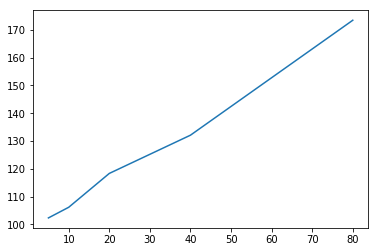
\includegraphics[scale=1]{Unknown1}}
            \caption{Brute plot of in-sample prediction error }
    \end{figure}
          
\end{homeworkProblem}




\begin{homeworkProblem}
Implement the following model (you can use any language)
\[
y_i=\beta^\ast_{[1]}x_{i[1]}+\beta^\ast_{[2]}x_{i[2]}+\epsilon_i
\]
where \(\mathbb{E}(\epsilon_i)=0\), \(\Var(\epsilon_i)=1\), \(\Cov(x_i,x_j)=0\) and \(\beta=(-1,2)^T\).  We also assume \(x_i\sim N(0,\Sigma_x)\) with
\[
\Sigma_x=\Cov(x_i)=\left(\begin{array}{cc} 1 & 0.9999\\ 0.9999 & 1 \end{array}\right)
\]
We repeated the following 2000 times:

    \begin{itemize}
        \item Generate \(\textbf{y}=(y_1, ..., y_{50})^T\) and \(\textbf{X}=(x_1, ..., x_{50})\).
        \item compute and record \(\hat{\beta}^{ols}\) and \(\hat{\beta}^{ridge}\).  What conclusion can you make from these histograms?
    \end{itemize}
Then report the followings:
     \begin{itemize}
        \item[$a.$] The histograms for \(\hat{\beta}^{ols}_{[1]}\) and \(\hat{\beta}^{ridge}_{[1]}\).  What conclusion can you make from these histograms?
        \item[$b.$] For each replicate of the 2000 repeats, compare \(\lvert\hat{\beta}^{\ast}_{[1]}-\hat{\beta}^{ols}_{[1]}\rvert\) with \(\lvert\beta^{\ast}_{[1]}-\beta^{ridge}_{[1]}\rvert\).  How many times does ridge regression return a better estimate of \(\beta^\ast_{[1]}\)?
     \end{itemize}
     
     \textbf{Solutions}
    \begin{figure}
            \centerline{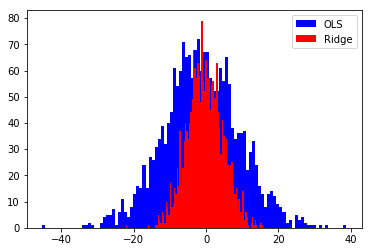
\includegraphics[scale=1]{Unknown}}
            \caption{Histogram for $\hat{\beta}_{[1]}^{ols}$ and $\hat{\beta}_{[1]}^{ridge}$}
    \end{figure}
           
    \textbf{a.} The predictions from OLS have a greater variance than those from Ridge, as shown in Figure 2. 
    
    \textbf{b.}
    Among the 2000 runs, \(\lvert\beta_{[1]}^\ast-\beta_{[1]}^{ridge}\rvert < \lvert\beta_{[1]}^\ast-\beta_{[1]}^{ols}\rvert\) for 1829 times.  That is, about 91.45\% of the times, ridge regression yields a better estimate compared to ordinary least square (OLS) regression.
          
\end{homeworkProblem}




\end{document}